\documentclass[8pt,aspectratio=169]{beamer}
\usetheme{Madrid}
\usepackage{graphicx}
\usepackage{booktabs}
\usepackage{adjustbox}
\usepackage{multicol}
\usepackage{amsmath}
\usepackage{amssymb}
\usepackage{listings}
\usepackage{xcolor}

% Color definitions
\definecolor{mlblue}{RGB}{0,102,204}
\definecolor{mlpurple}{RGB}{51,51,178}
\definecolor{mllavender}{RGB}{173,173,224}
\definecolor{mllavender2}{RGB}{193,193,232}
\definecolor{mllavender3}{RGB}{204,204,235}
\definecolor{mllavender4}{RGB}{214,214,239}
\definecolor{mlorange}{RGB}{255, 127, 14}
\definecolor{mlgreen}{RGB}{44, 160, 44}
\definecolor{mlred}{RGB}{214, 39, 40}
\definecolor{mlgray}{RGB}{127, 127, 127}

% Additional colors for template compatibility
\definecolor{lightgray}{RGB}{240, 240, 240}
\definecolor{midgray}{RGB}{180, 180, 180}

% Apply custom colors to Madrid theme
\setbeamercolor{palette primary}{bg=mllavender3,fg=mlpurple}
\setbeamercolor{palette secondary}{bg=mllavender2,fg=mlpurple}
\setbeamercolor{palette tertiary}{bg=mllavender,fg=white}
\setbeamercolor{palette quaternary}{bg=mlpurple,fg=white}
\setbeamercolor{structure}{fg=mlpurple}
\setbeamercolor{section in toc}{fg=mlpurple}
\setbeamercolor{subsection in toc}{fg=mlblue}
\setbeamercolor{title}{fg=mlpurple}
\setbeamercolor{frametitle}{fg=mlpurple,bg=mllavender3}
\setbeamercolor{block title}{bg=mllavender2,fg=mlpurple}
\setbeamercolor{block body}{bg=mllavender4,fg=black}

\setbeamertemplate{navigation symbols}{}
\setbeamertemplate{itemize items}[circle]
\setbeamertemplate{enumerate items}[default]
\setbeamersize{text margin left=5mm,text margin right=5mm}

\newcommand{\bottomnote}[1]{%
\vfill
\vspace{-2mm}
\textcolor{mllavender2}{\rule{\textwidth}{0.4pt}}
\vspace{1mm}
\footnotesize
\textbf{#1}
}

% TikZ and pgfplots packages
\usepackage{tikz}
\usepackage{pgfplots}
\pgfplotsset{compat=1.18}
\usetikzlibrary{arrows.meta, positioning, shapes.geometric, shapes.symbols, calc, decorations.pathmorphing, mindmap}

\title{Privacy \& Zero-Knowledge Proofs: A Visual Introduction}
\subtitle{Standalone Mini-Lecture}
\author{Prof.~Dr.~Joerg Osterrieder}
\institute{University Lecture Series}
\date{\today}
\begin{document}

% Frame 1: Title
\begin{frame}[plain]
\vfill
\begin{center}
{\Large\textbf{\textcolor{mlpurple}{Privacy \& Zero-Knowledge Proofs}}}\\[3mm]
{\large A Visual Introduction}\\[5mm]
{\footnotesize Prof.~Dr.~Joerg Osterrieder}\\[2mm]
{\footnotesize University Lecture Series}\\[5mm]
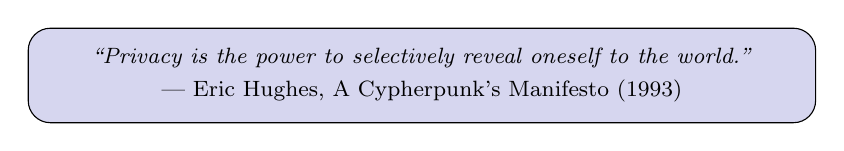
\begin{tikzpicture}
  \node[draw,fill=mllavender4,rounded corners=8pt,minimum width=10cm,minimum height=1.2cm,align=center] {
    \footnotesize\textit{``Privacy is the power to selectively reveal oneself to the world.''}\\
    \footnotesize --- Eric Hughes, A Cypherpunk's Manifesto (1993)
  };
\end{tikzpicture}
\end{center}
\vfill
\end{frame}

% Frame 2: What is a Zero-Knowledge Proof?
\begin{frame}{What is a Zero-Knowledge Proof?}
\begin{tikzpicture}[overlay,remember picture,shift={(current page.center)},
  panel/.style={draw=mlgray,rounded corners=6pt,fill=white,line width=0.5pt}]
  % Panel 1: The Scenario
  \node[panel,minimum width=3.8cm,minimum height=4.0cm] (p1) at (-5.2,0.2) {};
  \node[above,font=\scriptsize\bfseries,mlpurple] at (p1.north) {The Challenge};
  % Alice stick figure
  \draw[thick,mlblue] (-6.2,0.8) circle (0.25);
  \draw[thick,mlblue] (-6.2,0.55) -- (-6.2,-0.2);
  \draw[thick,mlblue] (-6.2,0.3) -- (-6.6,0) (-6.2,0.3) -- (-5.8,0);
  \draw[thick,mlblue] (-6.2,-0.2) -- (-6.5,-0.7) (-6.2,-0.2) -- (-5.9,-0.7);
  \node[font=\tiny,mlblue] at (-6.2,-0.95) {Alice};
  % Bob stick figure
  \draw[thick,mlorange] (-4.2,0.8) circle (0.25);
  \draw[thick,mlorange] (-4.2,0.55) -- (-4.2,-0.2);
  \draw[thick,mlorange] (-4.2,0.3) -- (-4.6,0) (-4.2,0.3) -- (-3.8,0);
  \draw[thick,mlorange] (-4.2,-0.2) -- (-4.5,-0.7) (-4.2,-0.2) -- (-3.9,-0.7);
  \node[font=\tiny,mlorange] at (-4.2,-0.95) {Bob};
  % Speech bubble
  \node[draw,fill=mllavender4,rounded corners,font=\tiny,align=center] at (-5.2,1.6) {Alice knows a secret\\but must prove it\\WITHOUT revealing it!};
  % Key icon
  \node[font=\large] at (-5.2,-1.3) {\textcolor{mlblue}{?}};

  % Panel 2: Three Properties
  \node[panel,minimum width=3.8cm,minimum height=4.0cm] (p2) at (-0.8,0.2) {};
  \node[above,font=\scriptsize\bfseries,mlpurple] at (p2.north) {Three ZK Properties};
  \node[draw,fill=mlgreen!15,rounded corners,minimum width=3cm,font=\tiny,align=center] at (-0.8,1.2) {\textbf{Completeness}\\If Alice is honest,\\Bob is always convinced};
  \node[draw,fill=mlorange!15,rounded corners,minimum width=3cm,font=\tiny,align=center] at (-0.8,0.0) {\textbf{Soundness}\\If Alice is cheating,\\Bob detects it};
  \node[draw,fill=mlblue!15,rounded corners,minimum width=3cm,font=\tiny,align=center] at (-0.8,-1.2) {\textbf{Zero-Knowledge}\\Bob learns NOTHING\\except that it's true};

  % Panel 3: Waldo Analogy
  \node[panel,minimum width=3.8cm,minimum height=4.0cm] (p3) at (3.6,0.2) {};
  \node[above,font=\scriptsize\bfseries,mlpurple] at (p3.north) {The Waldo Analogy};
  % Big sheet with hole
  \node[draw,fill=mllavender4,minimum width=3cm,minimum height=2.5cm,rounded corners] at (3.6,0.4) {};
  \node[draw,fill=mlred!30,circle,minimum size=0.6cm,font=\tiny\bfseries] at (3.6,0.4) {W};
  \node[font=\tiny,align=center] at (3.6,-0.8) {Cover the page with\\a sheet, cut a hole\\to show only Waldo};
  \node[font=\tiny,align=center,mlgreen!70!black] at (3.6,-1.4) {Proves you found him\\without revealing WHERE};
\end{tikzpicture}
\bottomnote{Zero-knowledge proofs are one of the most powerful tools in modern cryptography -- proving truth without information}
\end{frame}

% Frame 3: Interactive vs Non-Interactive Proofs
\begin{frame}{Interactive vs Non-Interactive Proofs}
\begin{tikzpicture}[overlay,remember picture,shift={(current page.center)},
  panel/.style={draw=mlgray,rounded corners=6pt,fill=white,line width=0.5pt}]
  % Panel 1: Interactive
  \node[panel,minimum width=3.8cm,minimum height=4.0cm] (p1) at (-5.2,0.2) {};
  \node[above,font=\scriptsize\bfseries,mlpurple] at (p1.north) {Interactive ZK};
  % Prover and Verifier with arrows
  \node[draw,fill=mlblue!15,rounded corners,minimum width=1cm,font=\tiny\bfseries] (pr1) at (-6.2,1.2) {Prover};
  \node[draw,fill=mlorange!15,rounded corners,minimum width=1cm,font=\tiny\bfseries] (vr1) at (-4.2,1.2) {Verifier};
  \draw[-{Stealth},mlblue,thick] (-5.9,0.8) -- (-4.5,0.8) node[midway,above,font=\tiny] {commit};
  \draw[-{Stealth},mlorange,thick] (-4.5,0.4) -- (-5.9,0.4) node[midway,above,font=\tiny] {challenge};
  \draw[-{Stealth},mlblue,thick] (-5.9,0.0) -- (-4.5,0.0) node[midway,above,font=\tiny] {response};
  \node[font=\tiny,align=center,mlgray] at (-5.2,-0.7) {Multiple rounds\\Both parties online\\Back-and-forth};
  \node[font=\tiny,align=center] at (-5.2,-1.3) {\textcolor{mlred}{Requires interaction}};

  % Panel 2: Non-Interactive (NIZK)
  \node[panel,minimum width=3.8cm,minimum height=4.0cm] (p2) at (-0.8,0.2) {};
  \node[above,font=\scriptsize\bfseries,mlpurple] at (p2.north) {Non-Interactive (NIZK)};
  \node[draw,fill=mlblue!15,rounded corners,minimum width=1cm,font=\tiny\bfseries] (pr2) at (-1.8,1.2) {Prover};
  \node[draw,fill=mlorange!15,rounded corners,minimum width=1cm,font=\tiny\bfseries] (vr2) at (0.2,1.2) {Verifier};
  \draw[-{Stealth},mlgreen,ultra thick] (-1.5,0.6) -- (-0.1,0.6) node[midway,above,font=\tiny\bfseries] {single proof};
  \node[draw,fill=mlgreen!15,rounded corners,font=\tiny,align=center] at (-0.8,-0.2) {Common Reference\\String (CRS)};
  \node[font=\tiny,align=center,mlgray] at (-0.8,-0.9) {One message\\Offline verification\\Blockchain-friendly};
  \node[font=\tiny,align=center] at (-0.8,-1.3) {\textcolor{mlgreen!70!black}{No interaction needed}};

  % Panel 3: Fiat-Shamir
  \node[panel,minimum width=3.8cm,minimum height=4.0cm] (p3) at (3.6,0.2) {};
  \node[above,font=\scriptsize\bfseries,mlpurple] at (p3.north) {Fiat-Shamir Transform};
  \node[draw,fill=mlblue!15,rounded corners,minimum width=2.5cm,font=\tiny,align=center] at (3.6,1.0) {Interactive\\Protocol};
  \draw[-{Stealth},mlpurple,ultra thick] (3.6,0.4) -- (3.6,-0.2);
  \node[draw,fill=mlorange!15,rounded corners,font=\tiny,align=center] at (3.6,0.1) {Replace verifier's\\challenge with\\hash function};
  \node[draw,fill=mlgreen!15,rounded corners,minimum width=2.5cm,font=\tiny,align=center] at (3.6,-0.8) {Non-Interactive\\Proof};
  \node[font=\tiny,align=center,mlgray] at (3.6,-1.4) {Hash = ``random oracle''};
\end{tikzpicture}
\bottomnote{The Fiat-Shamir heuristic (1986) converts any interactive proof to non-interactive -- essential for blockchain use}
\end{frame}

% Frame 4: The Math Behind ZK
\begin{frame}{The Math Behind ZK}
\begin{tikzpicture}[overlay,remember picture,shift={(current page.center)},
  panel/.style={draw=mlgray,rounded corners=6pt,fill=white,line width=0.5pt}]
  % Panel 1: Discrete Log (left, wider)
  \node[panel,minimum width=5.5cm,minimum height=4.0cm] (p1) at (-3.5,0.2) {};
  \node[above,font=\scriptsize\bfseries,mlpurple] at (p1.north) {Proving Without Revealing};
  % Padlock icon
  \node[draw,fill=mlblue!10,rounded corners,minimum width=4.5cm,align=center,font=\scriptsize] at (-3.5,1.0) {
    \textbf{Discrete Logarithm Problem}\\[1mm]
    Given $g$, $p$, and $y = g^x \bmod p$\\
    Finding $x$ is computationally hard
  };
  \node[draw,fill=mlgreen!15,rounded corners,minimum width=4.5cm,align=center,font=\tiny] at (-3.5,-0.2) {
    Alice can prove she \textbf{knows} $x$\\
    without ever sending $x$ to anyone!\\[1mm]
    This ``hardness assumption'' is the\\
    foundation of ZK proof security
  };
  \node[draw,fill=mlorange!10,rounded corners,minimum width=4.5cm,align=center,font=\tiny] at (-3.5,-1.3) {
    \textbf{Key idea:} Easy to verify ($g^x \stackrel{?}{=} y$)\\
    but hard to reverse (find $x$ from $y$)
  };

  % Panel 2: Commitment Schemes (right, wider)
  \node[panel,minimum width=5.5cm,minimum height=4.0cm] (p2) at (3.0,0.2) {};
  \node[above,font=\scriptsize\bfseries,mlpurple] at (p2.north) {Commitment Schemes};
  \node[draw,fill=mlblue!10,rounded corners,minimum width=4.5cm,align=center,font=\scriptsize] at (3.0,1.1) {
    \textbf{Pedersen Commitment}\\[1mm]
    $C = g^v \cdot h^r$\\[1mm]
    {\tiny $g, h$ = generators, $v$ = value, $r$ = randomness}
  };
  \node[draw,fill=mlgreen!15,rounded corners,minimum width=2cm,align=center,font=\tiny] at (1.5,-0.3) {
    \textbf{Hiding}\\[1mm]
    Cannot recover\\$v$ from $C$\\(info-theoretic)
  };
  \node[draw,fill=mlorange!15,rounded corners,minimum width=2cm,align=center,font=\tiny] at (4.5,-0.3) {
    \textbf{Binding}\\[1mm]
    Cannot change\\$v$ after commit\\(computational)
  };
  \node[draw,fill=mllavender4,rounded corners,minimum width=4.5cm,align=center,font=\tiny] at (3.0,-1.3) {
    Like a sealed envelope: you commit to a value\\
    without revealing it, but can't change it later
  };
\end{tikzpicture}
\bottomnote{Mathematical hardness assumptions (discrete log, pairings) make zero-knowledge proofs possible}
\end{frame}

% Frame 5: SNARKs vs STARKs
\begin{frame}{SNARKs vs STARKs}
\begin{tikzpicture}[overlay,remember picture,shift={(current page.center)},
  panel/.style={draw=mlgray,rounded corners=6pt,fill=white,line width=0.5pt}]
  % Panel 1: SNARKs
  \node[panel,minimum width=3.8cm,minimum height=4.0cm] (p1) at (-5.2,0.2) {};
  \node[above,font=\scriptsize\bfseries,mlblue] at (p1.north) {zk-SNARKs};
  \node[draw,fill=mlblue!10,rounded corners,minimum width=3.2cm,align=center,font=\tiny] at (-5.2,1.3) {
    \textbf{S}uccinct\\
    \textbf{N}on-interactive\\
    \textbf{AR}gument of\\
    \textbf{K}nowledge
  };
  \node[draw,fill=mlgreen!15,rounded corners,minimum width=3.2cm,font=\tiny,align=center] at (-5.2,0.0) {
    Proof size: \textbf{\textasciitilde200 bytes}\\
    Verification: \textbf{O(1)}\\
    Very fast to verify!
  };
  \node[draw,fill=mlred!15,rounded corners,minimum width=3.2cm,font=\tiny,align=center] at (-5.2,-1.0) {
    \textcolor{mlred}{Requires trusted setup}\\
    \textcolor{mlred}{Not quantum-safe}
  };

  % Panel 2: STARKs
  \node[panel,minimum width=3.8cm,minimum height=4.0cm] (p2) at (-0.8,0.2) {};
  \node[above,font=\scriptsize\bfseries,mlorange] at (p2.north) {zk-STARKs};
  \node[draw,fill=mlorange!10,rounded corners,minimum width=3.2cm,align=center,font=\tiny] at (-0.8,1.3) {
    \textbf{S}calable\\
    \textbf{T}ransparent\\
    \textbf{AR}gument of\\
    \textbf{K}nowledge
  };
  \node[draw,fill=mlgreen!15,rounded corners,minimum width=3.2cm,font=\tiny,align=center] at (-0.8,0.0) {
    No trusted setup!\\
    Post-quantum secure!\\
    Proof: \textbf{O(log$^2$ n)}
  };
  \node[draw,fill=mlorange!15,rounded corners,minimum width=3.2cm,font=\tiny,align=center] at (-0.8,-1.0) {
    \textcolor{mlorange}{Larger proofs (\textasciitilde45KB)}\\
    \textcolor{mlorange}{Heavier prover cost}
  };

  % Panel 3: Comparison
  \node[panel,minimum width=3.8cm,minimum height=4.0cm] (p3) at (3.6,0.2) {};
  \node[above,font=\scriptsize\bfseries,mlpurple] at (p3.north) {Head-to-Head};
  \node[font=\tiny] at (3.6,1.5) {
    \begin{tabular}{lcc}
    & \textbf{SNARK} & \textbf{STARK} \\
    \midrule
    Setup & Trusted & None \\
    Proof & \textasciitilde200B & \textasciitilde45KB \\
    Quantum & \textcolor{mlred}{No} & \textcolor{mlgreen}{Yes} \\
    Verify & Fast & Fast \\
    Prover & Fast & Slower \\
    \end{tabular}
  };
  \node[draw,fill=mllavender4,rounded corners,minimum width=3.2cm,font=\tiny,align=center] at (3.6,-0.6) {
    SNARKs: Zcash, zkSync\\
    STARKs: StarkNet, Cairo
  };
  \node[font=\tiny,align=center,mlpurple] at (3.6,-1.3) {Choose based on your\\trust \& quantum needs};
\end{tikzpicture}
\bottomnote{SNARKs trade trusted setup for tiny proofs; STARKs avoid trust assumptions but produce larger proofs}
\end{frame}

% Frame 6: Privacy Coins Overview
\begin{frame}{Privacy Coins Overview}
\begin{tikzpicture}[overlay,remember picture,shift={(current page.center)},
  panel/.style={draw=mlgray,rounded corners=6pt,fill=white,line width=0.5pt}]
  % Panel 1: Monero
  \node[panel,minimum width=3.8cm,minimum height=4.0cm] (p1) at (-5.2,0.2) {};
  \node[above,font=\scriptsize\bfseries,mlorange] at (p1.north) {Monero (XMR)};
  % Ring signature visual
  \node[draw,circle,fill=mlgray!20,minimum size=0.5cm,font=\tiny] (r1) at (-6.0,1.2) {?};
  \node[draw,circle,fill=mlgray!20,minimum size=0.5cm,font=\tiny] (r2) at (-5.2,1.5) {?};
  \node[draw,circle,fill=mlorange!30,minimum size=0.5cm,font=\tiny] (r3) at (-4.4,1.2) {\textbf{!}};
  \node[draw,circle,fill=mlgray!20,minimum size=0.5cm,font=\tiny] (r4) at (-5.2,0.7) {?};
  \draw[mlgray,thick] (r1) -- (r2) -- (r3) -- (r4) -- (r1);
  \draw[mlgray,thick] (r1) -- (r3) (r2) -- (r4);
  \node[font=\tiny,align=center] at (-5.2,0.0) {Ring signatures:\\real signer hidden\\among decoys};
  \node[draw,fill=mlorange!10,rounded corners,minimum width=3.2cm,font=\tiny,align=center] at (-5.2,-0.8) {
    + Stealth addresses\\
    + RingCT (hidden amounts)\\
    + Dandelion++ (network)
  };
  \node[font=\tiny,mlgreen!70!black] at (-5.2,-1.5) {\textbf{Default privacy for all}};

  % Panel 2: Zcash
  \node[panel,minimum width=3.8cm,minimum height=4.0cm] (p2) at (-0.8,0.2) {};
  \node[above,font=\scriptsize\bfseries,mlblue] at (p2.north) {Zcash (ZEC)};
  % Shielded pool visual
  \node[draw,fill=mlblue!5,rounded corners,minimum width=3cm,minimum height=1.5cm] at (-0.8,1.0) {};
  \node[font=\tiny\bfseries,mlblue] at (-0.8,1.5) {Shielded Pool};
  \node[draw,fill=white,rounded corners,font=\tiny] (ta) at (-1.8,0.5) {t-addr};
  \node[draw,fill=mlblue!20,rounded corners,font=\tiny] (za) at (0.2,0.5) {z-addr};
  \draw[-{Stealth},thick,mlblue] (ta) -- (za) node[midway,above,font=\tiny] {shield};
  \node[font=\tiny,align=center] at (-0.8,-0.3) {zk-SNARKs prove\\valid transactions\\without revealing details};
  \node[draw,fill=mlblue!10,rounded corners,minimum width=3.2cm,font=\tiny,align=center] at (-0.8,-1.0) {
    Transparent (t) or\\
    Shielded (z) addresses\\
    Opt-in privacy model
  };

  % Panel 3: Comparison
  \node[panel,minimum width=3.8cm,minimum height=4.0cm] (p3) at (3.6,0.2) {};
  \node[above,font=\scriptsize\bfseries,mlpurple] at (p3.north) {Monero vs Zcash};
  \node[font=\tiny] at (3.6,1.0) {
    \begin{tabular}{lcc}
    & \textbf{XMR} & \textbf{ZEC} \\
    \midrule
    Privacy & Default & Opt-in \\
    Crypto & Ring sig & SNARKs \\
    Setup & None & Trusted \\
    Tx size & \textasciitilde2KB & \textasciitilde2KB \\
    Audit & Hard & Possible \\
    \end{tabular}
  };
  \node[draw,fill=mllavender4,rounded corners,minimum width=3.2cm,font=\tiny,align=center] at (3.6,-0.5) {
    Both achieve strong\\privacy but via very\\different approaches
  };
  \node[font=\tiny,align=center,mlpurple] at (3.6,-1.3) {Different philosophy:\\always-on vs opt-in};
\end{tikzpicture}
\bottomnote{Monero uses ring signatures for default privacy; Zcash uses zk-SNARKs for optional shielded transactions}
\end{frame}

% Frame 7: ZK-Rollups Simplified
\begin{frame}{ZK-Rollups Simplified}
\begin{tikzpicture}[overlay,remember picture,shift={(current page.center)},
  panel/.style={draw=mlgray,rounded corners=6pt,fill=white,line width=0.5pt}]
  % Panel 1: The Problem
  \node[panel,minimum width=3.8cm,minimum height=4.0cm] (p1) at (-5.2,0.2) {};
  \node[above,font=\scriptsize\bfseries,mlred] at (p1.north) {The Problem};
  % Traffic jam of txs
  \foreach \i in {0,...,5} {
    \foreach \j in {0,...,2} {
      \node[draw,fill=mlred!20,minimum size=0.35cm,font=\tiny,inner sep=0] at (-6.0+\i*0.4, 1.2-\j*0.45) {tx};
    }
  }
  \node[draw,fill=mlred!30,rounded corners,minimum width=3.2cm,font=\tiny,align=center] at (-5.2,-0.3) {
    Ethereum L1:\\
    \textasciitilde15 TPS\\
    High gas fees\\
    Congested
  };
  \node[font=\tiny,mlred,align=center] at (-5.2,-1.2) {Cannot scale to\\millions of users};

  % Panel 2: The Solution
  \node[panel,minimum width=3.8cm,minimum height=4.0cm] (p2) at (-0.8,0.2) {};
  \node[above,font=\scriptsize\bfseries,mlgreen!70!black] at (p2.north) {ZK-Rollup Solution};
  % Funnel
  \foreach \i in {0,...,3} {
    \node[draw,fill=mlblue!15,minimum size=0.3cm,font=\tiny,inner sep=0] at (-1.5+\i*0.4, 1.5) {tx};
  }
  \foreach \i in {0,...,3} {
    \node[draw,fill=mlblue!15,minimum size=0.3cm,font=\tiny,inner sep=0] at (-1.5+\i*0.4, 1.1) {tx};
  }
  \draw[thick,mlpurple] (-1.7,0.8) -- (-0.8,0.2) -- (0.1,0.8);
  \node[draw,fill=mlgreen!20,rounded corners,minimum width=1.5cm,font=\tiny\bfseries,align=center] at (-0.8,-0.3) {ZK\\Proof};
  \draw[-{Stealth},thick,mlgreen!70!black] (-0.8,-0.7) -- (-0.8,-1.2);
  \node[font=\tiny,align=center] at (-0.8,-1.4) {Single proof\\on L1};

  % Panel 3: The Result
  \node[panel,minimum width=3.8cm,minimum height=4.0cm] (p3) at (3.6,0.2) {};
  \node[above,font=\scriptsize\bfseries,mlblue] at (p3.north) {The Result};
  \node[draw,fill=mlgreen!15,rounded corners,minimum width=3.2cm,font=\tiny,align=center] at (3.6,1.2) {
    \textbf{1000x throughput}\\
    Thousands of txs\\
    verified with one proof
  };
  \node[draw,fill=mlblue!10,rounded corners,minimum width=3.2cm,font=\tiny,align=center] at (3.6,0.0) {
    \textbf{Low gas cost}\\
    Proof verification\\
    is cheap on L1
  };
  \node[draw,fill=mllavender4,rounded corners,minimum width=3.2cm,font=\tiny,align=center] at (3.6,-1.0) {
    \textbf{Projects:}\\
    zkSync, StarkNet,\\
    Polygon zkEVM, Scroll
  };
\end{tikzpicture}
\bottomnote{ZK-Rollups batch thousands of transactions off-chain and post a single proof on-chain -- the future of scaling}
\end{frame}

% Frame 8: Real-World ZK Applications
\begin{frame}{Real-World ZK Applications}
\begin{tikzpicture}[overlay,remember picture,shift={(current page.center)},
  qbox/.style={draw=mlgray,rounded corners=6pt,fill=white,minimum width=5.0cm,minimum height=1.8cm,align=center,line width=0.5pt}]
  % Top-left: Private Voting
  \node[qbox] (q1) at (-3.2,1.4) {};
  \node[above left,font=\scriptsize\bfseries,mlpurple] at (q1.north east) {Private Voting};
  \node[font=\tiny,align=center] at (-3.2,1.4) {
    Anonymous but verifiable elections\\[1mm]
    Prove eligibility without revealing identity\\
    Prevent bribery \& coercion (MACI)
  };
  \node[font=\normalsize] at (-5.2,1.9) {\textcolor{mlblue}{$\square$}};

  % Top-right: Identity Verification
  \node[qbox] (q2) at (3.2,1.4) {};
  \node[above left,font=\scriptsize\bfseries,mlpurple] at (q2.north east) {Identity Verification};
  \node[font=\tiny,align=center] at (3.2,1.4) {
    Prove age $\geq$ 18 without showing ID\\[1mm]
    Self-sovereign identity (SSI)\\
    Selective disclosure of credentials
  };
  \node[font=\normalsize] at (1.2,1.9) {\textcolor{mlgreen}{$\diamondsuit$}};

  % Bottom-left: DeFi Privacy
  \node[qbox] (q3) at (-3.2,-1.0) {};
  \node[above left,font=\scriptsize\bfseries,mlpurple] at (q3.north east) {DeFi Privacy};
  \node[font=\tiny,align=center] at (-3.2,-1.0) {
    Private trading (no front-running)\\[1mm]
    Hidden balances \& amounts\\
    Railgun, Aztec, Penumbra
  };
  \node[font=\normalsize] at (-5.2,-0.5) {\textcolor{mlorange}{$\bigtriangleup$}};

  % Bottom-right: Supply Chain
  \node[qbox] (q4) at (3.2,-1.0) {};
  \node[above left,font=\scriptsize\bfseries,mlpurple] at (q4.north east) {Supply Chain};
  \node[font=\tiny,align=center] at (3.2,-1.0) {
    Prove product authenticity\\[1mm]
    Without exposing trade secrets\\
    Verify compliance privately
  };
  \node[font=\normalsize] at (1.2,-0.5) {\textcolor{mlred}{$\heartsuit$}};
\end{tikzpicture}
\bottomnote{ZK proofs enable ``verify without revealing'' across voting, identity, finance, and supply chains}
\end{frame}

% Frame 9: The ZK Landscape
\begin{frame}{The ZK Landscape}
\begin{tikzpicture}[overlay,remember picture,shift={(current page.center)},
  panel/.style={draw=mlgray,rounded corners=6pt,fill=white,line width=0.5pt}]
  % Left panel: Timeline
  \node[panel,minimum width=5.5cm,minimum height=4.0cm] (p1) at (-3.5,0.2) {};
  \node[above,font=\scriptsize\bfseries,mlpurple] at (p1.north) {ZK Evolution Timeline};
  % Timeline
  \draw[thick,mlgray] (-5.5,-1.5) -- (-5.5,1.8);
  \foreach \y/\yr/\evt in {
    1.6/1985/{GMR: ZK proofs defined},
    1.0/2012/{SNARKs constructed},
    0.4/2016/{Zcash launches},
    -0.2/2018/{STARKs published},
    -0.8/2020/{PLONK universal setup},
    -1.4/2023/{ZK-Rollups go live}} {
    \draw[thick,mlblue] (-5.7,\y) -- (-5.3,\y);
    \node[right,font=\tiny\bfseries,mlblue] at (-5.2,\y) {\yr};
    \node[right,font=\tiny] at (-4.4,\y) {\evt};
  }

  % Right panel: Ecosystem
  \node[panel,minimum width=5.5cm,minimum height=4.0cm] (p2) at (3.0,0.2) {};
  \node[above,font=\scriptsize\bfseries,mlpurple] at (p2.north) {ZK Ecosystem Map};
  \node[draw,fill=mlblue!15,rounded corners,minimum width=4.5cm,font=\tiny,align=center] at (3.0,1.3) {
    \textbf{Research:} Universities, IACR, Ethereum Foundation\\
    Zero-knowledge theory, new proof systems
  };
  \node[draw,fill=mlgreen!15,rounded corners,minimum width=4.5cm,font=\tiny,align=center] at (3.0,0.2) {
    \textbf{Infrastructure:} Circom, Noir, Cairo, Halo2, SP1\\
    Proving systems, compilers, developer tools
  };
  \node[draw,fill=mlorange!15,rounded corners,minimum width=4.5cm,font=\tiny,align=center] at (3.0,-0.9) {
    \textbf{Applications:} zkSync, StarkNet, Zcash, Worldcoin\\
    Rollups, privacy, identity, compliance
  };

  % Bottom summary bar
  \node[draw,fill=mllavender4,rounded corners,minimum width=11cm,font=\tiny\bfseries,align=center] at (0,-2.0) {
    ``ZK is the most important cryptographic breakthrough since public-key cryptography'' -- many researchers
  };
\end{tikzpicture}
\bottomnote{From a 1985 theory paper to production rollups in 2023 -- ZK technology is accelerating rapidly}
\end{frame}

% Frame 10: Key Takeaways
\begin{frame}{Key Takeaways}
\begin{tikzpicture}[overlay,remember picture,shift={(current page.center)},
  tbox/.style={draw=mlgray,rounded corners=6pt,fill=white,minimum width=5.0cm,minimum height=0.8cm,align=left,line width=0.5pt,font=\tiny}]
  % 5 numbered boxes
  \node[tbox,fill=mlblue!8] (b1) at (0,1.8) {
    \textbf{\textcolor{mlblue}{1.}} ZK proofs prove knowledge without revealing it -- completeness, soundness, zero-knowledge
  };
  \node[tbox,fill=mlgreen!8] (b2) at (0,0.8) {
    \textbf{\textcolor{mlgreen}{2.}} SNARKs are small but need trusted setup; STARKs are transparent and quantum-safe
  };
  \node[tbox,fill=mlorange!8] (b3) at (0,-0.2) {
    \textbf{\textcolor{mlorange}{3.}} Privacy coins (Monero, Zcash) use different cryptographic approaches to hide transactions
  };
  \node[tbox,fill=mlred!8] (b4) at (0,-1.2) {
    \textbf{\textcolor{mlred}{4.}} ZK-Rollups are scaling Ethereum by orders of magnitude using validity proofs
  };
  \node[tbox,fill=mlpurple!8] (b5) at (0,-2.2) {
    \textbf{\textcolor{mlpurple}{5.}} ZK powers private voting, identity verification, DeFi privacy, and supply chain integrity
  };
  % Coming next bar
  \node[draw,fill=mllavender4,rounded corners,minimum width=10cm,minimum height=0.6cm,align=center,font=\tiny\bfseries] at (0,-3.1) {
    Coming Next: Deep dive into proof system math, circuit design, privacy coin internals, and ZK-rollup architecture
  };
\end{tikzpicture}
\bottomnote{Zero-knowledge proofs are transforming blockchain scalability, privacy, and identity -- the future is provable}
\end{frame}

\end{document}
